\chapter{Introduzione}

La gestione dinamica della memoria è una delle principali responsabilità dei sistemi operativi moderni\footnotemark. La memoria ospita i processi attivi e i dati correntemente elaborati dal software in esecuzione; in quanto essa è più veloce da accedere dei dispositivi di memoria di massa, spesso viene usata come intermediario nella comunicazione che essi hanno con i processi. Con l'avvento dei sistemi multiprogrammati, la suddivisione della memoria in partizioni dedicate a ogni \textit{task} è diventata un aspetto principale dell'attività dei sistemi operativi: partizionare la memoria in aree contingentate rapidamente e efficacemente è un compito sfidante. 

\begin{quote}
“Memory is the new disk and disk is the new tape.”\\
\hfill --- Jim Gray
\end{quote}

\footnotetext{Dove per memoria si intende la \textit{Random Access Memory}, o RAM.}

Il sistema operativo si deve occupare di gestire e monitorare lo stato di ciascun indirizzo di memoria fisica, regolando l'allocazione della memoria tra i processi concorrenti, e definire le politiche di assegnazione, stabilendo quali processi possano accedere alla memoria, per quanto tempo e la quantità di memoria disponibile per ciascuno. Durante l'allocazione, il sistema operativo determina le specifiche locazioni di memoria da assegnare e ne mantiene traccia, aggiornandone lo stato in caso di rilascio o deallocazione. Un ulteriore aspetto che richiede attenzione è la memoria di cui il sistema operativo stesso ha necessità per svolgere le sue funzioni; poiché esso svolge numerosi compiti, laddove le strutture in atto per gestire le sue necessità di memoria siano lente o abbiamo un grande sovracosto ciò potrebbe portare a risultati disastrosi per la generale fluidità del calcolatore.

Quando la grandezza del programma è nota alla compilazione e non cambia, è semplice segnalare al sistema operativo quanta memoria sarà necessaria per tutto il ciclo di vita del programma. Questa memoria prende il nome di \textbf{staticamente allocata}. L'incarico di gestione risulta dunque semplificato: non sempre però è possibile determinare a priori le necessità del programma, in quanto queste potrebbero dipendere da vari fattori che non sono noti al programmatore (e.g. \textit{user input}). Un primo approccio, dispendioso e generalmente da evitare, consiste nell'allocare staticamente la memoria necessaria nel \textit{worst case scenario}: ossia prevedere in anticipo quale possa essere il bisogno di memoria più elevato nel corso della vita del programma e richiedere questa quantità. In questo modo però la memoria disponibile del sistema operativo potrebbe risultare nulla\footnotemark quando invece all'interno dei programmi ne esiste di non utilizzata al momento ed esistono casi per cui svolgere questo calcolo è impossibile, poiché il tetto massimo è imprevedibile. In generale questa pratica risulta impossibile da applicare in contesti dove la quantità di memoria non è abbondante.

\footnotetext{Out of memory (OOM) error}

L'alternativa risulta immediata, ma non di facile implementazione: fornire al programmatore sistemi per \textbf{allocare dinamicamente} la memoria, ossia per variare la grandezza dell'area dedicata ai dati del programma durante la sua vita, ingrandendola e restringendola in base alle necessità. In questo modo, memoria viene occupata solamente quando è necessaria e nel momento in cui non è più utile viene restituita al sistema operativo, che può assegnarla a un altro programma. L'allocazione della memoria consiste dunque nell'identificare un blocco di memoria libera di dimensione adeguata per soddisfare una richiesta. Le allocazioni di memoria vengono gestite attingendo da un'area contigua denominata \textit{heap} (o \textit{free store}). 

\begin{figure}[H]
  \centering
  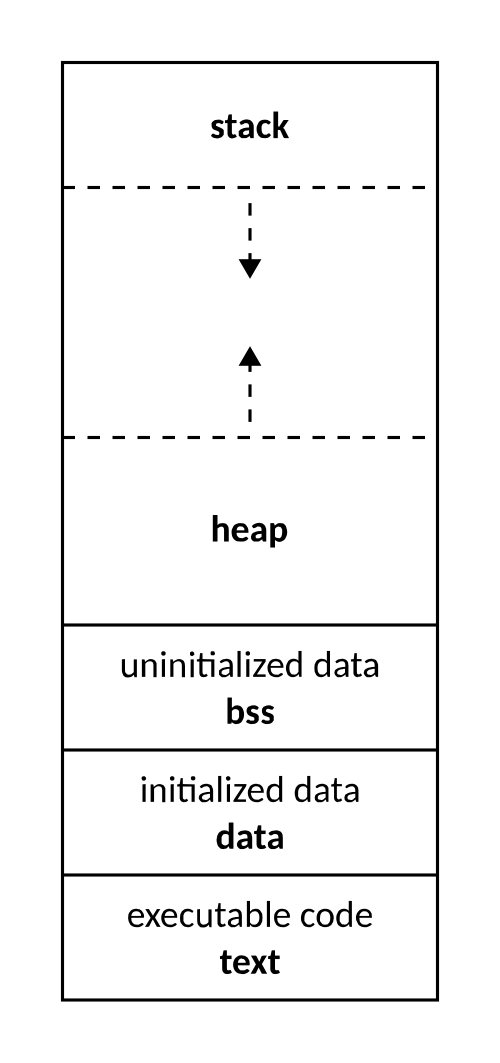
\includegraphics[width=0.2\textwidth]{images/program_memory_layout.png}
  \caption{Layout semplificato della memoria di un programma.}
  \label{fig:program_memory_layout}
\end{figure}

\paragraph{Allocazione manuale o automatica della memoria.}
Linguaggi di programmazione diversi gestiscono questa problematica secondo principalmente due paradigmi: l'allocatore può funzionare in modo manuale, ossia rispondendo alla chiamata esplicita di funzioni che comunicano le necessità del programma, o in modo automatico, attraverso \textit{garbage collectors}. Questi ultimi consistono in un insieme di \textit{routine} che determinano se esiste memoria il cui riferimento viene perso all'interno del programma e che dunque sono irraggiungibili e li aggiungono alla memoria disponibile. Esistono diversi meccanismi per effettuare questa analisi, ma nel corso della nostra analisi ci concentreremo sull'allocazione manuale di memoria, in particolare nelle modalità in cui avviene nel linguaggio di programmazione \textbf{C}. 

\section{\textit{Memory Allocators}}

In un dato istante, alcune regioni dell'\textit{heap} sono riservate (in uso da parte di processi o strutture dati), mentre altre rimangono libere (non allocate) e pertanto disponibili per esaudire future richieste. Il \textit{Memory Allocator} è il modulo specializzato del sistema operativo che sovrintende all'assegnazione e al rilascio di questa risorsa. All'inizializzazione dell'allocatore viene assegnata per il suo uso una quantità di memoria; esso si occupa dunque di gestirla dinamicamente. Ciò può avvenire secondo strategie e politiche ben diverse: obiettivo di questo progetto è l'esplorazione di un sottoinsieme rappresentativo di questi moduli, caratterizzati da un campione delle suddette strategie, evidenziando nelle loro implementazioni i benefici e i punti deboli.

Il programma dell'utente manipola o muta lo stato della memoria. L'allocatore non ha alcuna informazione sulla memoria, sul suo contenuto o sul suo ciclo di vita e, una volta assegnata della memoria, deve rispettare le indicazioni dell'utente. In altre parole, l'algoritmo di allocazione è online e possiede informazioni limitate, con cui svolge delle valutazioni seguendo euristiche di comportamento. Nei capitoli successivi verranno analizzati in dettaglio alcuni di questi algoritmi, con particolare attenzione alle loro implementazioni pratiche e ai contesti applicativi in cui risultano più efficaci. 

\paragraph{Allocatori a user level.} 
Generalmente, quando facciamo riferimento a un gestore di memoria, parliamo di una componente del sistema operativo, che ha dunque privilegi diversi e un grado maggiore di autonomia rispetto a un programma in svolgimento. Tuttavia, non è irragionevole pensare che per un utente gestire autonomamente la memoria possa essere utile in determinati contesti: ad esempio, in applicazioni embedded o real-time, dove è fondamentale garantire tempi di risposta prevedibili, una gestione personalizzata della memoria può migliorare le prestazioni. In altri casi, come nei database o nei sistemi ad alte prestazioni, allocatori specializzati possono ottimizzare l'uso della memoria per specifiche modalità di accesso, riducendo l'overhead e aumentando l'efficienza complessiva del sistema. Nel corso del progetto, particolare attenzione è stata posta nel sottolineare in quali situazioni un determinato approccio sia più vantaggioso.

\section{Svolgimento del progetto}
L'obiettivo di questo progetto è duplice: da una parte vedremo i benefici che possono essere ricavati dalla scelta oculata delle corrette strategie in base alle proprie necessità, senza affidarsi a soluzioni generiche, dall'altra illustreremo le opportunità che l'analisi accurata dei propri programmi attraverso l'uso di strumenti preesistenti, ma anche oppure di propria creazione, fornisce ai programmatori. Nessuno può conoscere le esigenze di gestione dinamica della memoria di un programma come il suo creatore e, per quanto possano essere brillanti le euristiche adoperate in assenza di ulteriori dati, è appropriato che egli scelga e, laddove sia necessario, implementi una soluzione \textit{ad hoc} piuttosto che affidarsi a un sistema generico.

Nel secondo capitolo, esploriamo la letteratura accademica alla base delle scelte progettuali, senza scendere nel dettaglio su specifiche implementazioni degli algoritmi di allocazione, ma acquistando una visuale storica e contestuale dell'allocazione dinamica di memoria. Approfondiamo le motivazioni per cui esistono riserve e preoccupazioni sull'allocazione dinamica di memoria in determinate applicazioni. Citando articoli rilevanti, stabiliamo le basi formali per le valutazioni del lavoro svolto. Forniamo quindi risorse utili per acquisire informazioni sull'argomento anche per chi si trovi ad affrontarlo per la prima volta e menzioniamo le opere che sono state d'ispirazione. 

In seguito descriviamo i gestori di memoria sviluppati nel corso del progetto, declinati in tre tipologie principali: lo \texttt{SlabAllocator}, il \texttt{BuddyAllocator} e il \texttt{BitmapBuddyAllocator}. Analizziamo le tecniche adoperate e giustifichiamo le scelte progettuali e implementative prese nel contesto didattico del corso di Sistemi Operativi. Esplicitiamo dunque quali siamo le metriche d'interesse per valutare la performance degli allocatori: stabiliamo contemporaneamente le nostre aspettative riguardo i risultati che ci aspettiamo di riscontrare.
Nel capitolo successivo, infatti, ci occupiamo dapprima di valutare la correttezza degli allocatori, attraverso una serie di test che ci forniscano la certezza che essi si comportino come desiderato, ma in secondo luogo poniamo le basi per un analisi più approfondita creando un linguaggio che possiamo adoperare per descrivere formalmente un benchmark. 
L'unico modo infatti di poter fare una scelta consapevole è riflettere attentamente sulle proprie necessità e indagare a fondo i procedimenti per acquisire un'intuizione dei costi e dei \textit{trade-off}.
Una volta fatto ciò, osserviamo i risultati e li confrontiamo con le ipotesi fatte durante la descrizione dell'implementazione, valutando il comportamento e l'efficacia della nostra soluzione e cercando di spiegare eventuali fenomeni imprevisti. 